\chapter{Introduction}

This document is a portfolio for CS4157, Software Quality, taught by Dr. Ita Richardson. It aims to illustrate and summarise the key concepts explored, and the learning process, within the module. Each week will be a briefly summary of the key points that I took from the lectures, and a discussion on any papers, and how useful, or useless, I found them. Summaries of meetings held by the group tasked with the module project will also be listed. 

\chapter{Week 1}
\section{Learnings}

The three key things I took from this weeks lecture were:

\begin{enumerate}
\item Eliminate testing by refining process
\begin{itemize}
\item By following a quality process and focusing on quality throughout, the need for testing can be reduced.
\end{itemize}
\item Other things in software system
\begin{itemize}
\item Be ware of other items in the software system: hardware, users, environment etc
\end{itemize}
\item Problem based learning
\begin{itemize}
\item Tackle the issue and learn how to solve the problem by working on the problem
\end{itemize}
\end{enumerate}

\section{Paper}

The paper that was looked at this week was "Understanding the implementation of software process improvement innovations in software organisations" \parencite{week1}. The goal of the paper is to "achieve a better understanding of the processes influencing the introduction, organizational implementation and adoption of software process improvement innovations in and by software companies" \parencite{week1}.

I found the paper a bit difficult to read, as it focused on a number of research methodologies that I am not familiar with, but I did like the breakdown on types of innovation.

\textbf{Individualistic Perspective} assumes that single individuals  that the main source of innovation within an organisational structure. Actions by these people are "not seen to be constrained by external factors" \parencite{week1}. These individuals are self guiding, and focused, and any decisions they make are made in order to "maximise value or utility" \parencite{week1}

\textbf{Structuralist Perspective} assumes that "innovation is determined by objectively existing organizational characteristics" \parencite{week1}. This view seems to place the chance of innovation on factors within the organisation, such as an "organisations size, its task structure differentiation, its task complexity, its employees job specialization and their professionalism" \parencite{week1}.	 

\textbf{Interactive Process Perspective} assumes innovation is "dynamic, continuous phenomenon of change over time" that is a result of both individual and organisational factors \parencite{week1}. It focuses on the interactions between individual and organisations. Innovation is the result of the "continuous interaction of the actions of individuals, structural influences and innovation itself" \parencite{week1}.

\section{Meeting}

No meeting held this week.

\chapter{Week 2}

\section{Learnings}

\begin{enumerate}
\item Quality priority depends on perspective
\begin{itemize}
\item I defined quality as the amount of reliability that a product or service has
\end{itemize}
\item When is it really important to ensure high quality?
\begin{itemize}
\item The output, where it is being used? - Example: salt from fast food dissolved seat belts. All possibilities cannot be tested for!
\end{itemize}
\item 'Good Enough' software - for the purpose it is built for
\begin{itemize}
\item Functions are right, the cycle time is right, the quality is right, development productivity is right - capability of process.
\end{itemize}
\end{enumerate}

\section{Paper}

\section{Meeting}
\chapter{Week 3}

\section{Learnings}
\begin{enumerate}
\item Project Capability
\begin{itemize}
\item
\end{itemize}
\item Project Maturity
\begin{itemize}
\item
\end{itemize}
\item Total Quality Management
\begin{itemize}
\item
\end{itemize}
\end{enumerate}

\section{Paper}

\section{Meeting}
\chapter{Week 4}

\section{Learnings}
\begin{enumerate}
\item Improved process leads to improved product
\begin{itemize}
\item
\end{itemize}
\item Regulations for software
\begin{itemize}
\item FDA in America, EU directives within the EU.
\end{itemize}
\item
\begin{itemize}
\item
\end{itemize}
\end{enumerate}

\section{Paper}

\section{Meeting}
\chapter{Week 5}

\section{Learnings}
\begin{enumerate}
\item Business importance of software increasing
\begin{itemize}
\item 90\% of the cost of a car is software
\end{itemize}
\item Business Benefits
\begin{itemize}
\item Return on investment increases, productivity increases, overall effect decrease. More money, less work with a good process.
\end{itemize}
\item Software Process Improvement
\begin{itemize}
\item Productivity up, Defects down, Error Rates down, Costs down, On Time Deliverables up, Rework down and savings in test time. 
\end{itemize}
\item Software Process Models
\begin{itemize}
\item Capability Maturity Model, ISO 15504, Configuration Management, Assessment of System
\end{itemize}
\end{enumerate}

\section{Paper}

\section{Meeting}
\chapter{Week 6}

\section{Learnings}
\begin{enumerate}
\item
\begin{itemize}
\item
\end{itemize}
\item
\begin{itemize}
\item
\end{itemize}
\item
\begin{itemize}
\item
\end{itemize}
\end{enumerate}

\section{Paper}

\section{Meeting}

\chapter{Week 7}

\section{Learnings}
\begin{enumerate}
\item
\begin{itemize}
\item
\end{itemize}
\item
\begin{itemize}
\item
\end{itemize}
\item
\begin{itemize}
\item
\end{itemize}
\end{enumerate}

\section{Paper}

\section{Meeting}

\section{Question Prep}
\begin{enumerate}
\item How difficult is it to integrate a connected health solution with an existing system?
\item Failures in connected health system? How are failures handled? Repercussions?
\item Integration of IT and Healthcare - What usability issues arise and how are they handled?
\end{enumerate}

\chapter{Week 8}

\section{Learnings}
\begin{center}
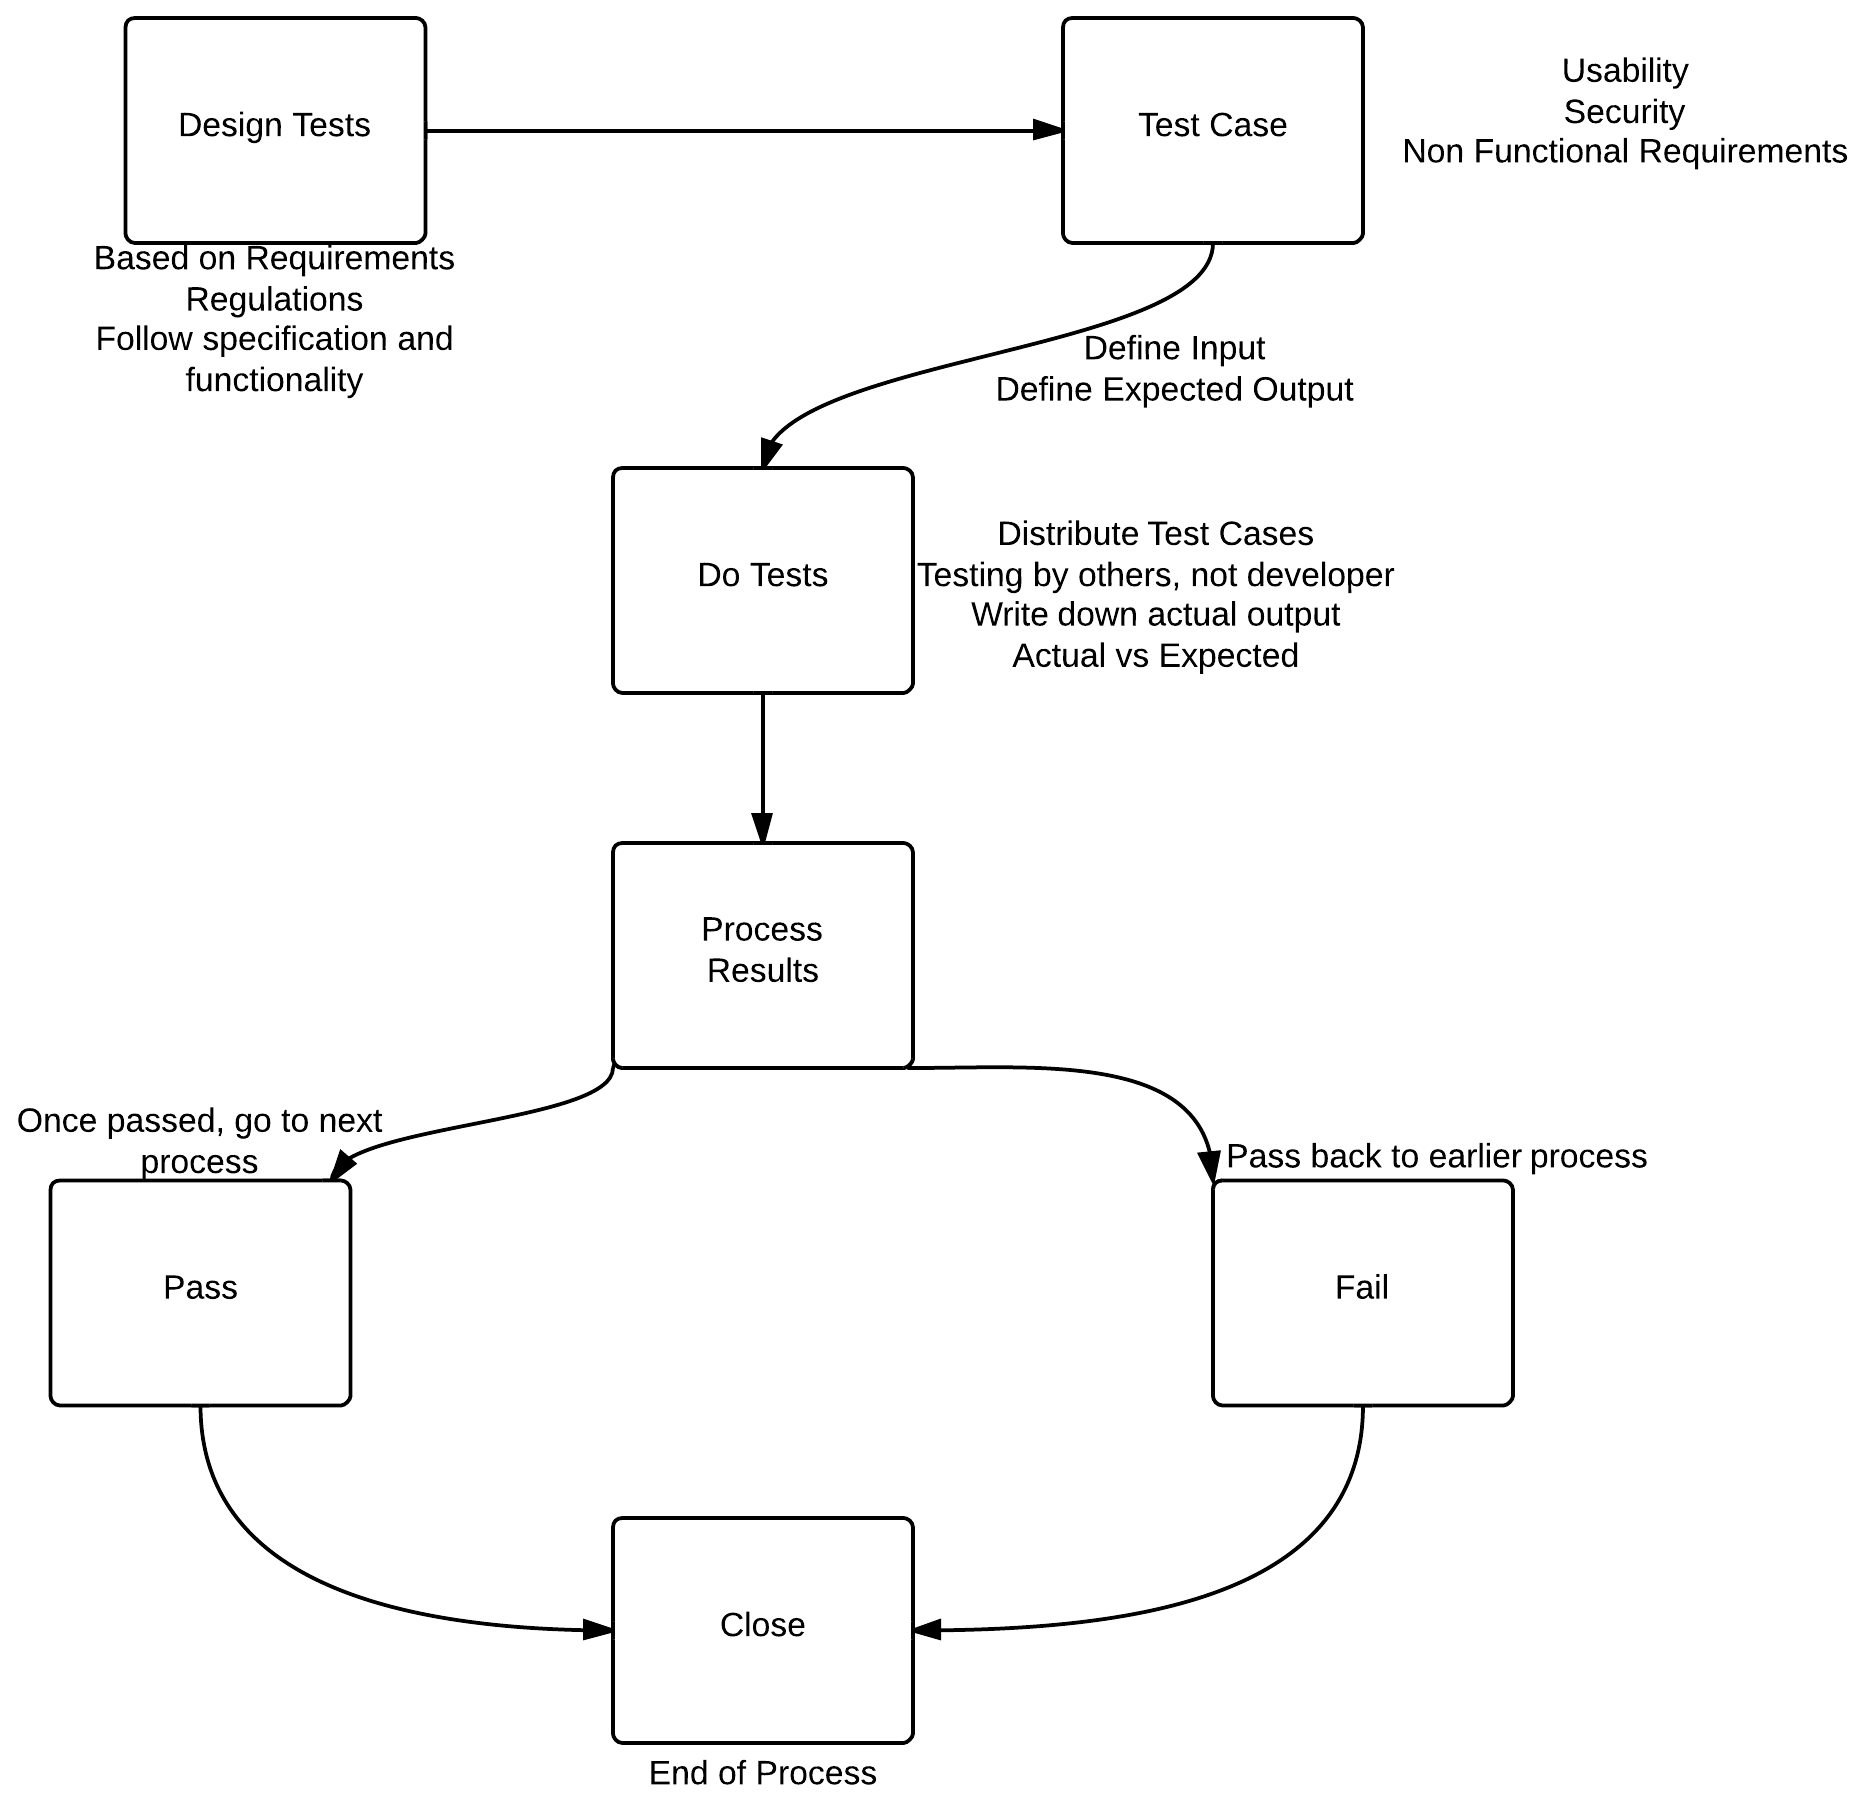
\includegraphics[scale=0.3]{testing.png}
\end{center}


\section{Paper}

\section{Meeting}
\chapter{Week 9}

\section{Learnings}
\begin{enumerate}
\item
\begin{itemize}
\item
\end{itemize}
\item
\begin{itemize}
\item
\end{itemize}
\item
\begin{itemize}
\item
\end{itemize}
\end{enumerate}

\section{Paper}

\section{Meeting}
\chapter{Week 10}

\section{Learnings}
\begin{enumerate}
\item FYPs are stressful
\begin{itemize}
\item
\end{itemize}
\item The lab is pretty hot on demo day
\begin{itemize}
\item
\end{itemize}
\item After demo day, any food seems like mana from heaven
\begin{itemize}
\item
\end{itemize}
\end{enumerate}

\section{Paper}

\section{Meeting}
\chapter{Week 11}

\section{Learnings}
\begin{enumerate}
\item
\begin{itemize}
\item
\end{itemize}
\item
\begin{itemize}
\item
\end{itemize}
\item
\begin{itemize}
\item
\end{itemize}
\end{enumerate}

\section{Paper}

\section{Meeting}
\chapter{Week 12}

\section{Learnings}
\begin{enumerate}
\item
\begin{itemize}
\item
\end{itemize}
\item
\begin{itemize}
\item
\end{itemize}
\item
\begin{itemize}
\item
\end{itemize}
\end{enumerate}

\section{Paper}

\section{Meeting}


